\documentclass[12pt,letterpaper]{article}
\usepackage[utf8]{inputenc}
\usepackage[english]{babel}
\usepackage{ragged2e}
\usepackage[colorlinks = true,
            linkcolor = purple,
            urlcolor  = blue,
            citecolor = blue,
            anchorcolor = blue]{hyperref}
\hypersetup{
    colorlinks=true,
    linkcolor=blue,
    filecolor=blue,      
    urlcolor=blue,} 
\urlstyle{same}


\usepackage{ifpdf}
\usepackage{mla}

\begin{document}

\begin{mla}{Michael}{Brodskiy}{Mrs. Greer}{AP Language}{October 8, 2020}{\underline{Analyzing Political Cartoons}} 

  \begin{justifying}

    \paragraph{I.} In S.J. Ray's and K.C. Star's cartoon entitled, ``The Rude Awakening,'' Adolf Hitler is depicted in a dazed, perturbed state as a result of the Eastern front closing in. The bear in this figure serves the purpose of a hyperbolic metaphor, the symbol of Russians, the predominant ethic subculture of the former Soviet Union. Jaws wide open ready to snap and questioning Hitler's ``\emph{intuition}'', in reference to the defeat of the German Sixth Army and the following Westward push by Soviet Armies.
    \paragraph{II.} In this cartoon Hitler is pictured in bed, frightened and in an inherently vulnerable position while the behemoth labeled Russia stares at him menacingly. The bear, with its mouth open, displaying two rows of jagged teeth, taunts Hitler's inevitable series of defeats starting in early 1943. Hitler's ``\emph{intuition}'', \textit{blitzkrieg}, which enabled his armies to traverse the European republics of the Soviet Union failed to be efficient in the long-run, \textit{rattenkrieg}, which took it's place, did not allow the German armies to rely on Hitler's ``\emph{intuition}'' in the rubble of the many ruined Soviet cities. This composition serves not only as a symbol of shame and defeat in the present, but also a foreboding warning for the future, which would see the collapse of the Nazist regime at the hands of the Soviet Union.
    \paragraph{III.} This image's intent is clear $-$ it is meant to mock the dwindling Nazist regime $-$ ultimately causing a decline in morale. The ominous bear, hungry for a meal (i.e. \emph{victory}), is much like the Soviet Union. The bed in which Hitler is laying in has a double representation, as both Hitler and the Soviet bear were awaken. As such, by awakening the bear, the cartoon argues that Hitler has raised a force to be reckoned with. The expression of sheer horror on Hitler's face exemplifies the premonition of destruction and conveys the idea that he realized his ``\emph{intuition}'' had gone too far. Ergo, Ray's and Star's cartoon would be not only a prediction of the short-term future, but also the decades of tension to come, with the great awakening of an industrially dominant superpower regime.


    \begin{figure}[h]
      \centering
      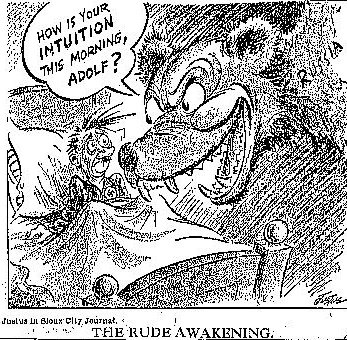
\includegraphics[width=.6\textwidth]{../Figures/Stalingrad.jpg}
      \caption{Ray, S.J. and Star, K.C. ``The Rude Awakening'' [\textit{illegible}] City Journal, 1943}
      \label{fig:1}
    \end{figure}


\end{justifying}
\centering Word Count: 345

\end{mla}

\end{document}

